% Chapter 3

\chapter{Computational model} % Main chapter title
\label{chapter:computationalmodel} % For referencing the chapter elsewhere, use \ref{Chapter1} 

The previous chapter, presented the experimental model designs for the iFEM process of the material 
parameter identification, detailing the experimental setups, results, and main assumptions 
made for the material models. These foundations enabled the development of the finite element (FE) model.

In this chapter, the computational models of the indentation tests introduced in Chapter \ref{chapter:experimentalmodel} 
will be described. These models were constructed using the finite element software ANSYS. 
The computational model serves as the principal link between the experimental data and the identification of the 
specimen's material parameters.\\  

The initial simulation model, referred to as Computational model I (CM I), served as a tool 
for testing the preliminary ideas, as well as establishing the basis structure for 
the computational model. This first step was essential to identify the strengths and 
weaknesses of the model, offering insights that guided the development of an 
improved simulation model, referred to as Computational model II (CM II). By examining the 
results and challenges of computational model I, the initial conceptual ideas for FE model 
were iterated, leading to the creation of a more robust and accurate computational model
for the material parameters' identification process.

In this chapter, the development process of the computational models will be discussed in detail, 
including the complications encountered, the proposed solutions, 
and the improvements made in computational model II.

%-----------------------------------------------------------------------------------------
\section{Computational model I}
\label{section:cpI}
\subsection{Middle Point}
\label{subsection:mpcpI}
The quasi-static nature of the indentation experiment for allowed the use of a static 
structural analysis. To prioritize the development of the framework for the material 
parameter identification process, the model was simplified as much as possible.
This approach minimized the influence of errors arising from complex geometries and boundary conditions.

\subsubsection*{Description}
The geometry only included key components that significantly contribute to the mechanical response,
i.e., the indenter and the specimen. The tumor extraction geometry depicted in Figure \ref{fig:specimenhole}
was also modeled for CM I. Both the indenter and the specimen utilized SOLID187 elements.
SOLID187 elements are a high order 3-D, \SI{10}{}-node elements with three degrees of freedom at each node.
These elements were suitable for simulating deformations of nearly incompressible hyperelastic materials 
and offered hyperelasticity, large deflection, and large strain capabilities \cite{Ansys2010}.\\
%Geometry model CPI
The geometry model used for EM I is shown in Figure \ref{fig:geometrycpI}. %figure of the middle point geometry for experimental model I
Although symmetry could have been applied, it was not employed in this case. This decision considered 
future projects, where the measurement and identification of human organ material parameters were desired 
objectives. For these cases, due to the material's anisotropy and the usual complex geometry,
symmetry boundary conditions could not be applied. 
\begin{figure}%
    \centering
   \quad
   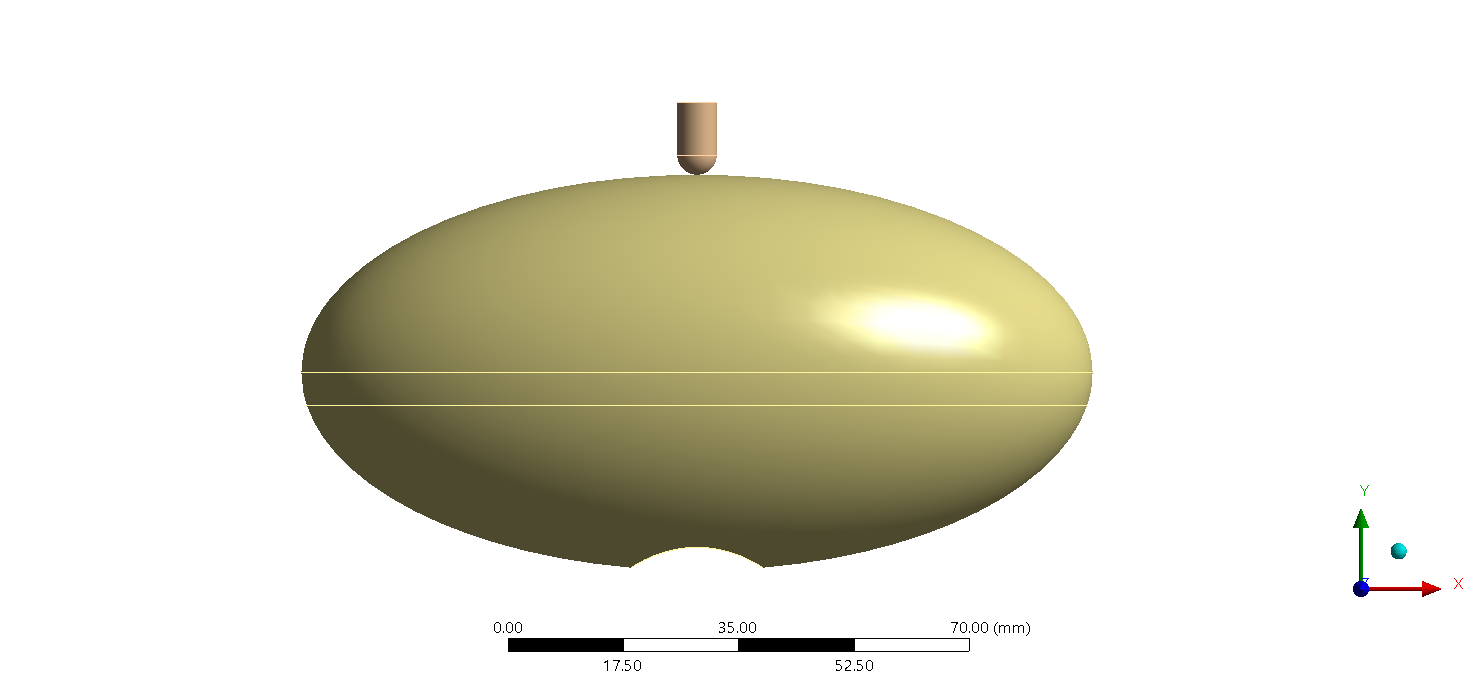
\includegraphics[width=10cm]{Images/computational/Assemblynoplatform2.png}%
   \caption[Computational model I geometry]{CM I geometry: Illustration of the geometry model with its key components, indenter and specimen with tumor extraction.}%
   \label{fig:geometrycpI}%
\end{figure}
%contact
The contact formulation between the indenter and the specimen was set to frictionless (CONTA174) to reduce
overall model complexity and mimic the lubricated contact of the experiment configuration.
The lower half of the specimen was defined as a fixed support, mirroring the physical constraint of the 
experimental setup. The displacement value $h$ was applied to the indenter in the Y-direction,
and the force reaction $F$ was subsequently obtained.\\
%Mesh
A global element size of $e_{I_s}=\SI{5}{\milli\meter}$ was applied to the specimen's mesh, which 
consisted of quadratic tetrahedral elements. The contact area between the indenter and the specimen's surface 
was refined to $e_{I_a}=\SI{0.3}{\milli\meter}$ (Fig.\ref{fig:cpImesh}). The primary reason for applying contact
sizing refinement was to ensure independence from the specimen's geometry or the indenter's position on the specimen's surface.\\
\begin{figure}
    \centering
    \begin{subfigure}[b]{0.45\textwidth}
    \centering
    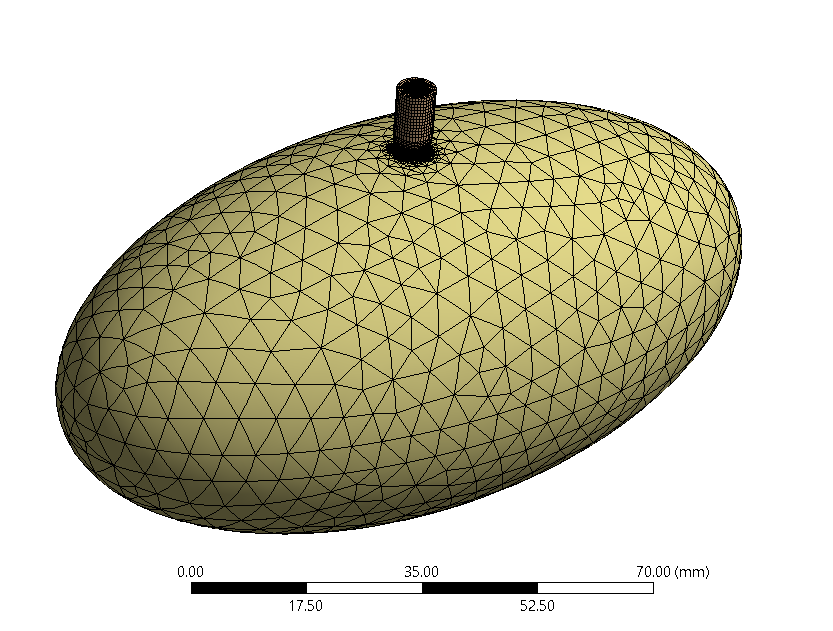
\includegraphics[width=\textwidth]{Images/computational/MeshCSES03total.png}
    \caption{Whole geometry meshing}
    \label{fig:cp1meshtotal}
    \end{subfigure}
    \hfill
    \begin{subfigure}[b]{0.45\textwidth}
    \centering
    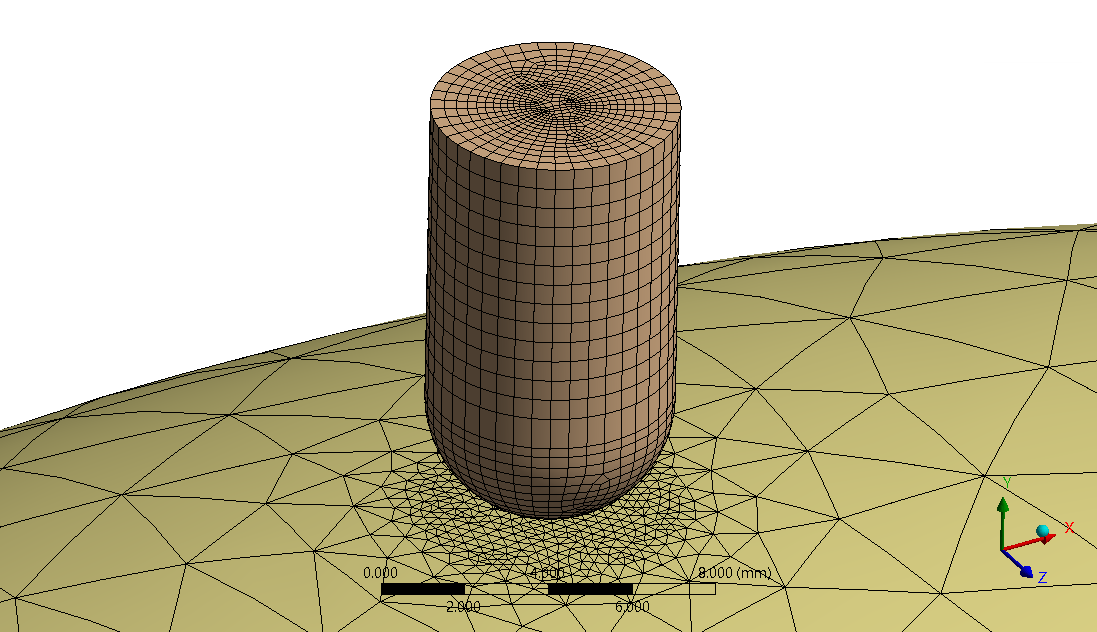
\includegraphics[width=\textwidth]{Images/computational/MeshCSES03.png}
    \caption{Mesh refinement area}
    \label{fig:cp1meshref}
    \end{subfigure}
    \hspace{0.3cm}
    \caption[Computational model I mesh]{CM I mesh: Patch conforming mesh with contact sizing refinement in the contact between the indenter and the specimen's surface.}
    \label{fig:cpImesh}
\end{figure}
Finally, initial parameters were assigned to the computational model to approximate the mechanical properties of ultra-soft polyurethane. 
For the linear elasticity level, values for the Young's modulus $E$ and the Poisson's ratio $\nu$ were assigned. 
From the main assumptions made in Section \ref{section:mainassumption}, the Poisson's ratio for the first 
level material model was set to $\nu_{LE} =  0.49$, and the Young's modulus was calculated using equation \ref{eq:forcelinear}
\begin{align}
    E = \frac{3F(1-\nu^2)} {4{r_i}^{\frac{1}{2}} {h}^{\frac{3}{2}}}\, .
    \label{eq:forcelinearcp1}
\end{align}
Substituting the indenter radius $r_i = \SI{3}{\milli \meter}$ and the indentation depth $h = \SI{3.8}{\milli \meter}$ a Young's modulus $E_{LE}$ was calculated and resulted in 
\begin{align}
    E_{LE} = 0.018 MPa \approx 0.02 MPa \, .
    \label{eq:Elinearcp1}
\end{align}


\subsubsection*{Level 1 Results}
\label{subsection:level1cmI}
An indentation depth of $h = \SI{3.8}{\milli \meter}$ could not be solved with the linear elastic material model. 
Through an iterative process, it was discovered that the linear elastic material model could only be applied 
up to an indentation depth of $h \approx \SI{2}{\milli \meter}$.\\

The initial attempt to match the experimental and simulation data provided a reasonable approximation of the experimental data.
Figure \ref{fig:MPI2mmvsCPILE} demonstrates the comparison between the experimental data and the CM I using a 
linear elastic material model up to an indentation depth of $h = \SI{2}{\milli \meter}$. The CM I curve displayed 
a more pronounced curvature than the experimental data. Additionally, at $u =\SI{0}{\milli \meter}$, 
the experimental curve exhibited a steeper initial slope; however, as the displacement increased, the 
difference in slope between the two curves diminished.\\

This result indicated that for a displacement greater than $u = \SI{2}{\milli \meter}$, the CM I curve would 
lie above the experimental data. Interestingly, it was observed that, despite employing a linear elastic model, 
the force-displacement curve exhibited a nonlinear response. This observation suggested that even a relatively 
simple material model could capture some degree of nonlinearity. 

\begin{figure}%
    \centering
   \quad
    \begin{tikzpicture}[scale=1]
        \begin{axis}[
            xmax=2.2,xmin=0,
            ymin= 0,ymax=0.2,
            %ytick={0,0.1,0.2,...,0.6},
            xlabel={Displacement $u [mm]$},
            ylabel={Force reaction $F_{MP} [N]$},
            grid = major,
            legend pos= north west]
            \addplot+[smooth, no markers, thick] table [y=$Force$, x=Def]{Table/CP1/MPI2mm.dat};
            \addplot+[smooth, no markers, thick] table [y=$Force$, x=Def]{Table/CP1/CP12mmCSfullmodelLE.dat};
            \legend{Experiment I,CM I-LE}
        \end{axis}
    \end{tikzpicture}%
   \caption[Computational model I vs. Experimental data - Linear elasticity]{CM I vs. EM I: Comparison of force-displacement curves between experimental data for Middle Point case and the initial computational model with a linear elastic model for $h = \SI{2}{\milli \meter}$.}%
   \label{fig:MPI2mmvsCPILE}%
\end{figure}


\subsubsection*{Level 2 Results}
\label{subsection:level2cmI}
At the hyperelastic level, the initial parameters for the Neo-Hookean model, 
the shear modulus $\mu$ and the incompressibility parameter $D_1$ were calculated from the Young's modulus $E_{LE}$
and the Poisson's ratio $\nu$ from the linear elastic model. With equations \ref{eq:mucp1}, \ref{eq:bulkmodcp1}, 
and \ref{eq:incomparcp1}, the shear modulus $\mu_{CMI}$ and the incompressibility parameter $D_{1_{CMI}}$
\begin{align}
    \mu_{CMI} = 0.0067 MPa \, ,
    \label{eq:mucp1result}
\end{align}
\begin{align}
    D_{1_{CMI}} = 6 MPa^{-1} \, ,
    \label{eq:d1cp1result}
\end{align}
were calculated, respectively. These parameters were integrated in the model described above. In comparison to 
the linear elastic model, the Neo-Hookean material model could solve the simulation for an indentation depth of 
$h =  \SI{3.7}{\milli \meter}$.
\begin{figure}%
    \centering
   \quad
    \begin{tikzpicture}[scale=1]
        \begin{axis}[
            xmax=4.2,xmin=0,
            ymin= 0,ymax=0.6,
            ytick={0,0.1,0.2,...,0.5},
            xlabel={Displacement $u [mm]$},
            ylabel={Force reaction $F_I [N]$},
            grid = major,
            legend pos= north west]
            \addplot+[smooth, no markers, thick] table [y=$Force$, x=Def]{Table/Middle Point/MPI38mm.dat};
            \addplot+[smooth, no markers, thick] table [y=$Force$, x=Def]{Table/CP1/CP1CSfullmodelNH.dat};
            \legend{Experiment I,CM I-NH}
        \end{axis}
    \end{tikzpicture}%
   \caption[Computational model I vs. Experimental data - Neo-Hookean]{CM I vs. EM I: Comparison of force-displacement curves between experimental data for Middle Point case and the initial computational model with a Neo-Hookean model for $h = \SI{3.8}{\milli \meter}$.}%
   \label{fig:MPIvsCPINH}%
\end{figure}
The Neo-Hookean simulation curve displayed a similar slope at lower values of $u$ in comparison to the experimental data.
As the displacement $u$ increased, the difference in slope between the two curves increased, and from $u \approx \SI{2.5}{\milli \meter}$
until the end, the computational curve showed a flatter slope than the experimental curve.\\

Despite the discrepancies between the two curves, the Neo-Hookean provided a fair approximation to the experimental data, considered the 
given displacement range. Likewise, this outcome evidenced that the Neo-Hookean model was capable of capturing some of the nonlinear 
response observed in the experimental data, by directly inputting the calculated values from the linear elastic material model.
Nevertheless, it is important to note that improvements to the computational model are necessary to achieve a more
accurate representation of the experimental results.

\subsection{Nearby Point}
For the nearby point test configuration described in Subsection \ref{subsection:nearbypoint} was also modeled to gain an insight 
of the first set material parameters obtained from the middle point computational model.
For the nearby point computational model, the Neo-Hookean model was employed, and the CM I was adapted by changing the 
indenter's position.

The experimental data curve from \ref{subsection:nearbypointresult} and the computational model's curve are shown in Figure 
\ref{fig:nbpointIvsCPINBNH}. Both curves exhibited a similar parabolic shape; however, the simulation curve showed once again,
at a larger indentation depth, a flatter slope than the experimental data. This result presented a 
nearly identical behavior to that of the middle point case.\\
\label{subsection:nbpcpI}
\begin{figure}%
    \centering
   \quad
    \begin{tikzpicture}[scale=1]
        \begin{axis}[
            xmax=4,xmin=0,
            ymin= 0,ymax=0.6,
            ytick={0,0.1,0.2,...,0.5},
            xlabel={Displacement $u [mm]$},
            ylabel={Force reaction $F_I [N]$},
            grid = major,
            legend pos= north west]
            \addplot+[smooth, no markers, thick] table [y=$Force$, x=Def]{Table/Nearby Point/nbexpI.dat};
            \addplot+[smooth, no markers, thick] table [y=$Force$, x=Def]{Table/CP1/NBPCSNHCPI.dat};            
            \legend{Nearby Point, CM I-NBP-NH}
        \end{axis}
    \end{tikzpicture}%
   \caption[Nearby Point: CM I vs. Experimental data - Neo-Hookean]{NBP - CM I vs. EM I: Comparison of force-displacement curves between experimental data for Nearby Point case and the initial computational model with a Neo-Hookean model for $h = \SI{3.8}{\milli \meter}$.}%
   \label{fig:nbpointIvsCPINBNH}%
\end{figure}
In conclusion, while there were differences, the initial calculated values provided a consistent approximation to experimental
data, indicating that the computational model captures the essential features of the material's behavior.
It was decided that further refinements of the material parameters may be necessary to minimize the error between the 
simulated and experimental curves.

%--------------------------------------------------------------------------------------------------------------
\section{Analysis and Complications}
\label{section:challengescm}
\subsection{Verification of the Computational Model}
The verification of the computational model was an important aspect of ensuring the accuracy and reliability of the 
simulation results. One typical approach to verify the model is to conduct a mesh convergence analysis. To 
reduce computational time, symmetry boundary conditions were applied, and one-quarter of CM I was used.

\subsubsection*{Mesh Convergence Analysis}
The mesh convergence FE model utilized a global element size $e_{M_s}=\SI{2}{\milli\meter}$ for the specimen
and $e_{M_i}=\SI{0.3}{\milli\meter}$ for the indenter.
A refinement was made in the area of interest, i.e., the contact area between the indenter and the specimen's surface,
with a sphere radius of $r_{M_a}=\SI{10}{\milli\meter}$ and an element size of $e_{M_a}=\SI{0.5}{\milli\meter}$ (Fig. \ref{fig:meshconvergencecmI}).

\begin{figure}%
    \centering
   \quad
   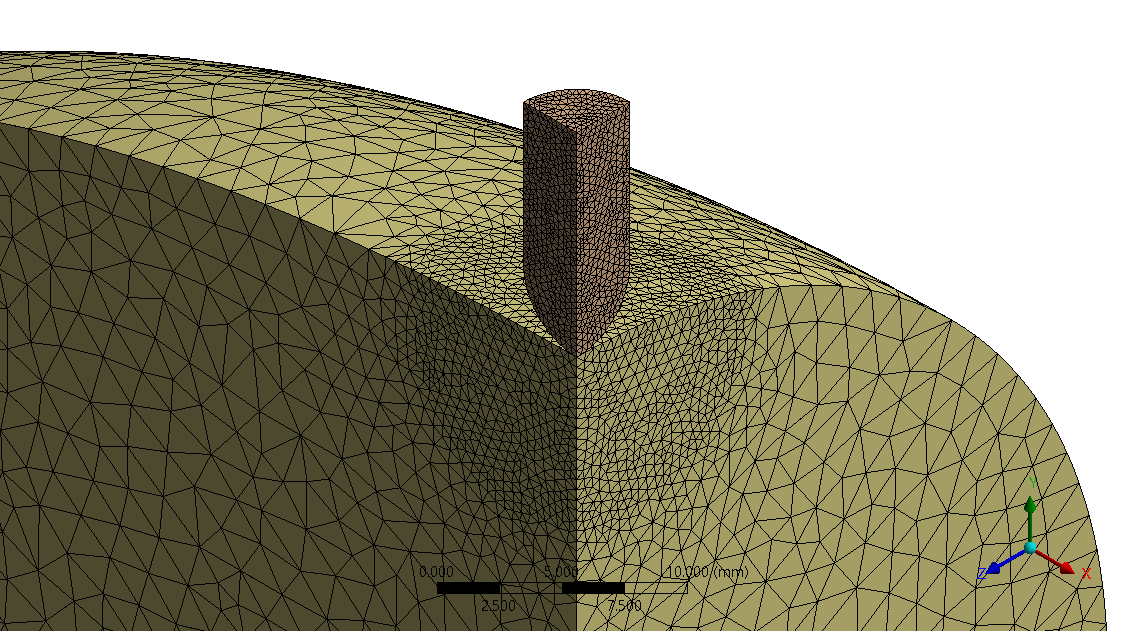
\includegraphics[width=10cm]{Images/computational/meshzoom.png}%
   \caption[Mesh convergence model I]{Mesh convergence analysis I: Mesh refinement strategy in the contact between the indenter and the specimen's surface using one-quarter of the model.}%
   \label{fig:meshconvergencecmI}%
\end{figure}

The mesh convergence analysis presented challenges, as reducing the element size from \SI{5}{\milli\meter} to 
\SI{0.1}{\milli\meter} in the contact area led to unsolvable cases due to large element deformation problems, 
or resulted in values deviating significantly from the expected convergence trend. However, a certain tendency 
towards convergence was observed.

\subsubsection*{Stress Distribution Analysis}
The second challenge encountered during the verification process was the analysis of the stress distribution in 
computational model I. A classic indentation solution between an almost rigid body and an elastic body gives a Hertzian 
solution \cite{Lin2009}. The expected Hertzian stress distribution was not clearly observed; instead, the stress 
contour plot showed rough borders, with some irregularities in the indentation surface area. This issue highlighted
the need for model improvement (Fig. \ref{fig:stressdistributionanalysis}).

Of interest was to observe a cleaner Hertzian stress distribution in the mesh convergence FE model as shown in Figure, 
suggesting that the original model was not entirely reliable and the mesh dependency in the contact area.  

\begin{figure}
    \centering
    \begin{subfigure}[b]{0.7\textwidth}
    \centering
    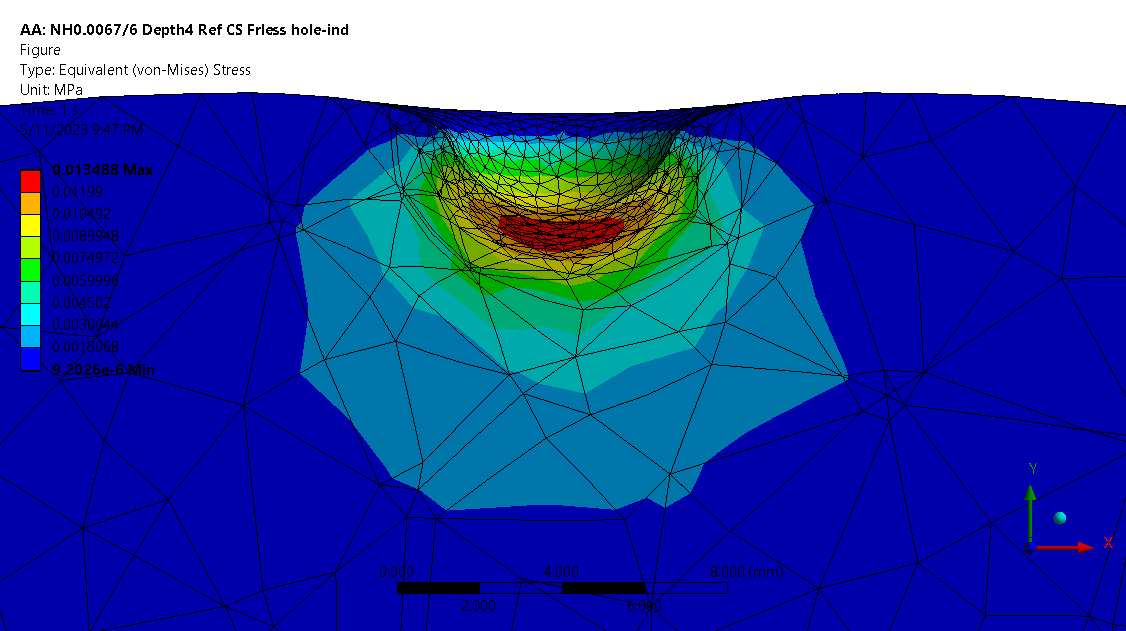
\includegraphics[width=\textwidth]{Images/computational/37CSNHstresshalfzoommesh.png}
    \caption{CM I - NH}
    \label{fig:cm1meshtotal}
    \end{subfigure}
    \vspace{0.3cm}
    \begin{subfigure}[b]{0.7\textwidth}
    \centering
    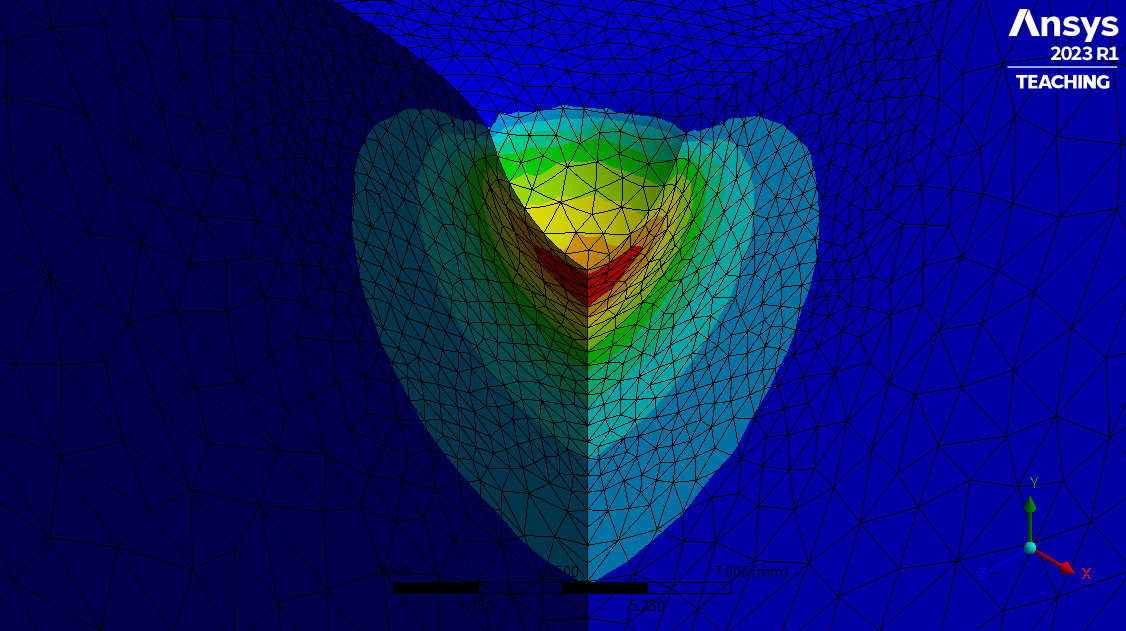
\includegraphics[width=\textwidth]{Images/computational/meshzoomstress.png}
    \caption{Mesh convergence model}
    \label{fig:cm1meshref}
    \end{subfigure}
    \hspace{0.3cm}
    \caption[Mesh convergence model I stress distribution]{Stress distribution analysis of the CM I with a Neo-Hookean material model and the mesh convergence model, which shows the irregularities in the stress contour plot.}
    \label{fig:stressdistributionanalysis}
\end{figure}
%----------------------------------------------------------------------------------------------------------------------
\section{Computational model II}
\label{section:cmII}
The computational model II or improved computational model, addressed the challenges and observations 
encountered during the development of CM I. This refined model integrated the proposed
solutions to the previously identified irregularities, and thus served as the final model for the 
iFEM approach for parameter identification. 

\subsection{Middle Point}
\label{subsection:mpcmII}
\subsubsection*{Description}
%geometry and contact
The CM II is the FE model of the experimental model II. The geometry model remained similar to CM I,
featuring a spherical indenter and specimen. The tumor extraction characteristic was omitted, as the 
lower part of the specimen was deemed irrelevant for the overall results (Fig. \ref{fig:cm2meshtotal}). Furthermore, in CM II, only 
one-half of the model was used, again taking advantage of the symmetry boundary conditions. Also,
this choice was made to facilitate the visualization of the deformation profile for subsequent validation 
steps. Same as in CM I, the contact set as frictionless, and the fixed support was applied to the lower part of the organ.\\

%mesh 
The mesh refinement for CM II was guided by the results of the mesh convergence analysis of CP I.
The global element size was maintained at $e_{{II}_s}=\SI{5}{\milli\meter}$, while the refinement area
was adjusted to $e_{{II}_a}=\SI{0.5}{\milli\meter}$ with a sphere radius of $r_{{II}_a}=\SI{8}{\milli\meter}$.
The results in CM I showed that the indenter could be considered as a rigid body; therefore, the element size was 
set at $e_{{II}_i}=\SI{1}{\milli\meter}$, as it did not have a significant influence on the results.
To further improve the mesh quality, a patch independent method was employed, reducing the mesh's 
maximum skewness from \SI{0.85}{} to \SI{0.6}{} (Fig. \ref{fig:cm2meshref}).
\begin{figure}
    \centering
    \begin{subfigure}[b]{0.45\textwidth}
    \centering
    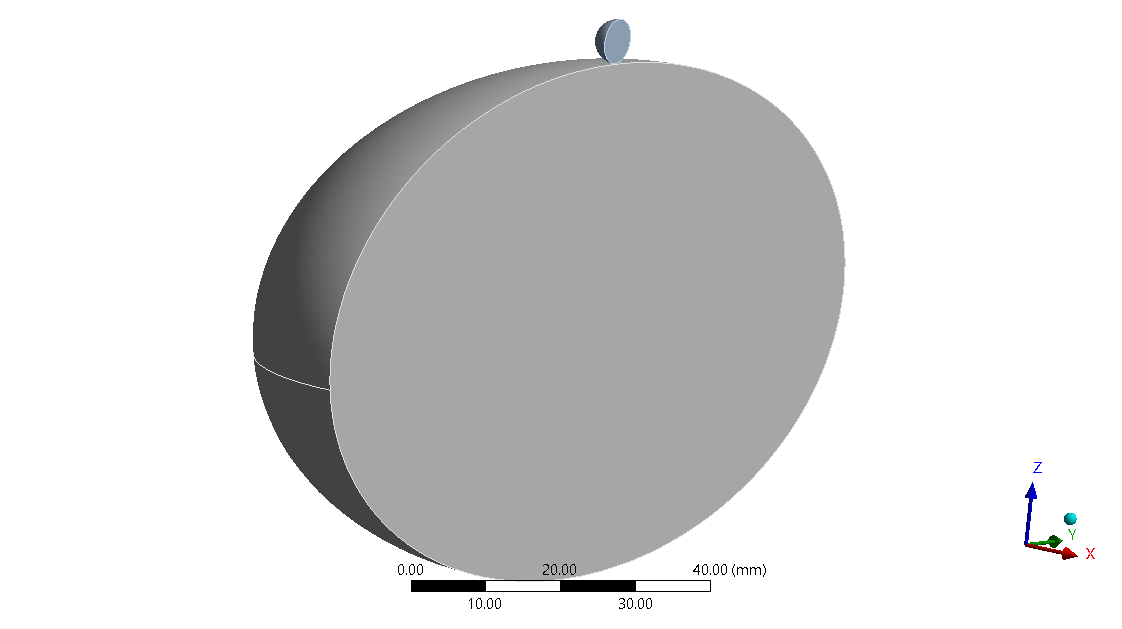
\includegraphics[width=\textwidth]{Images/computational/cm2geometry.png}
    \caption{Geometry model}
    \label{fig:cm2meshtotal}
    \end{subfigure}
    \hfill
    \begin{subfigure}[b]{0.45\textwidth}
    \centering
    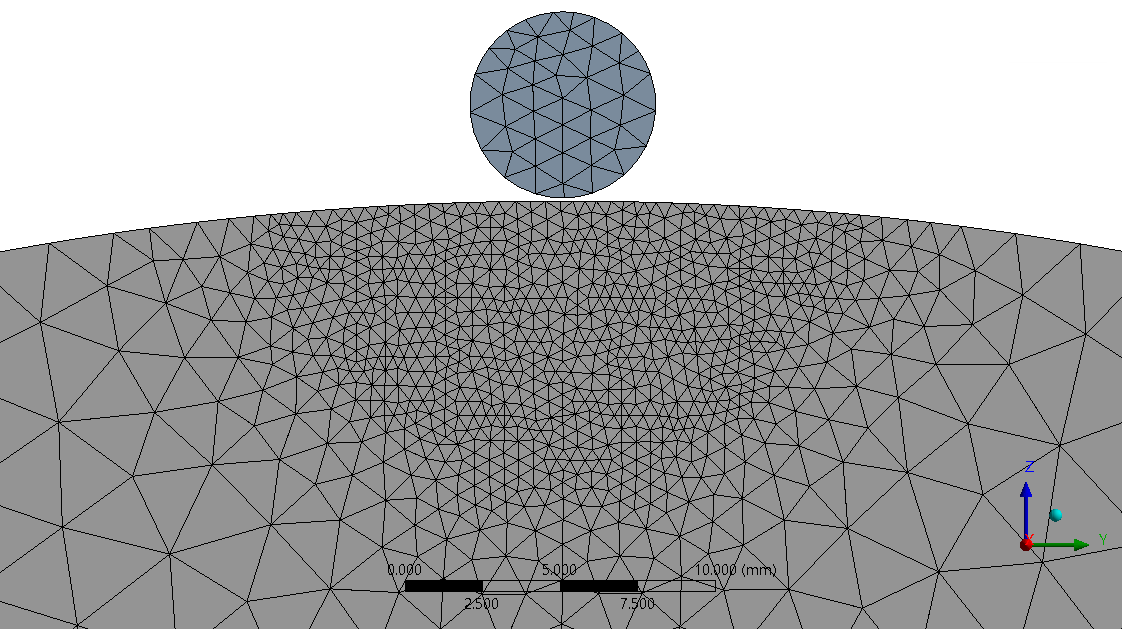
\includegraphics[width=\textwidth]{Images/computational/cm2meshzoom.png}
    \caption{Mesh refinement area}
    \label{fig:cm2meshref}
    \end{subfigure}
    \hspace{0.3cm}
    \caption[Computational model II mesh]{CM II mesh: Patch independent mesh with refinement in the contact area between the indenter and the specimen's surface.}
    \label{fig:cmIImesh}
\end{figure}

\subsubsection*{Large Element Deformation Strategy}
To address the issue of the large element deformation for larger indentation depths, the ANSYS \textbf{nonlinear adaptive region}
option was applied. This feature performed a remeshing operation in the contact area of the specimen whenever 
the elements reached a high distortion level. This adaptive meshing region process made it possible to conduct 
a successful mesh convergence analysis. In this mesh convergence analysis, all values could be calculated and 
convergence was reached. As a result, the element size in the contact area was determined to be changed from 
\SI{0.5}{\milli\meter} to \SI{1}{\milli\meter}. 

\subsubsection*{Stress Distribution Strategy}
In terms of the stress distribution, the computational model II demonstrated improvements over CM I. The new
stress contour plot exhibited more clearly defined borders, and the irregularities present in CM I did not 
emerge on the specimen's indented surface. This resulted in a stress distribution that more closely aligned
with the expected Hertzian solution. A comparative illustration of the stress distributions from CM I and 
CM II is displayed in Figure \ref{fig:cmIIstressdistanalysis}.\\

\begin{figure}
    \centering
    \begin{subfigure}[b]{0.7\textwidth}
    \centering
    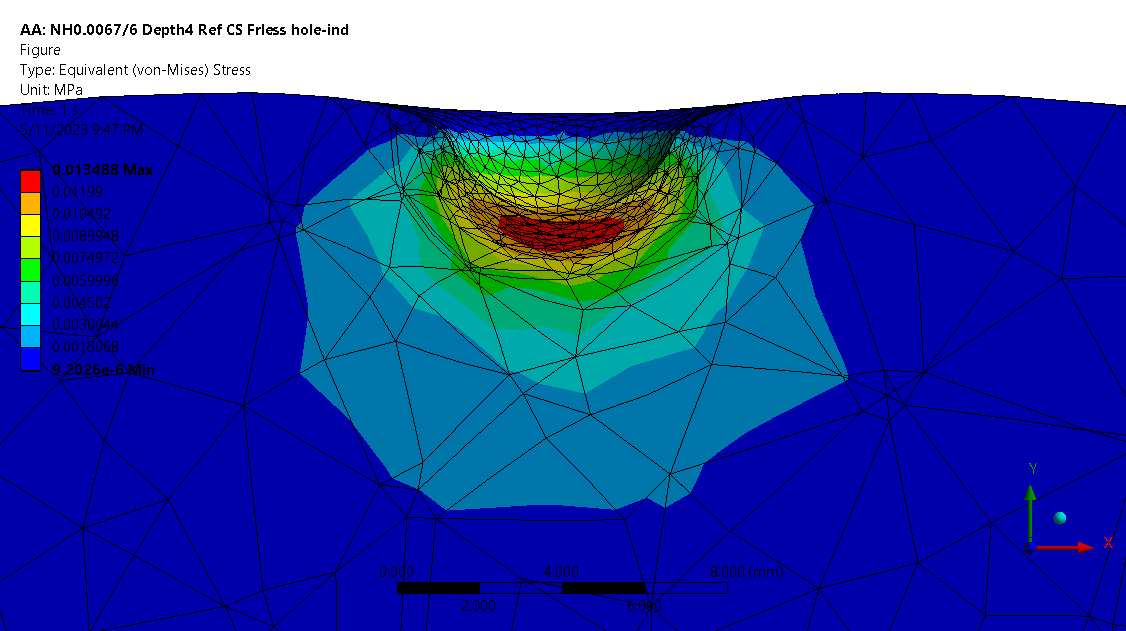
\includegraphics[width=\textwidth]{Images/computational/37CSNHstresshalfzoommesh.png}
    \caption{Computational model I}
    \label{fig:cm1stress}
    \end{subfigure}
    \hspace{0.3cm}
    \begin{subfigure}[b]{0.7\textwidth}
    \centering
    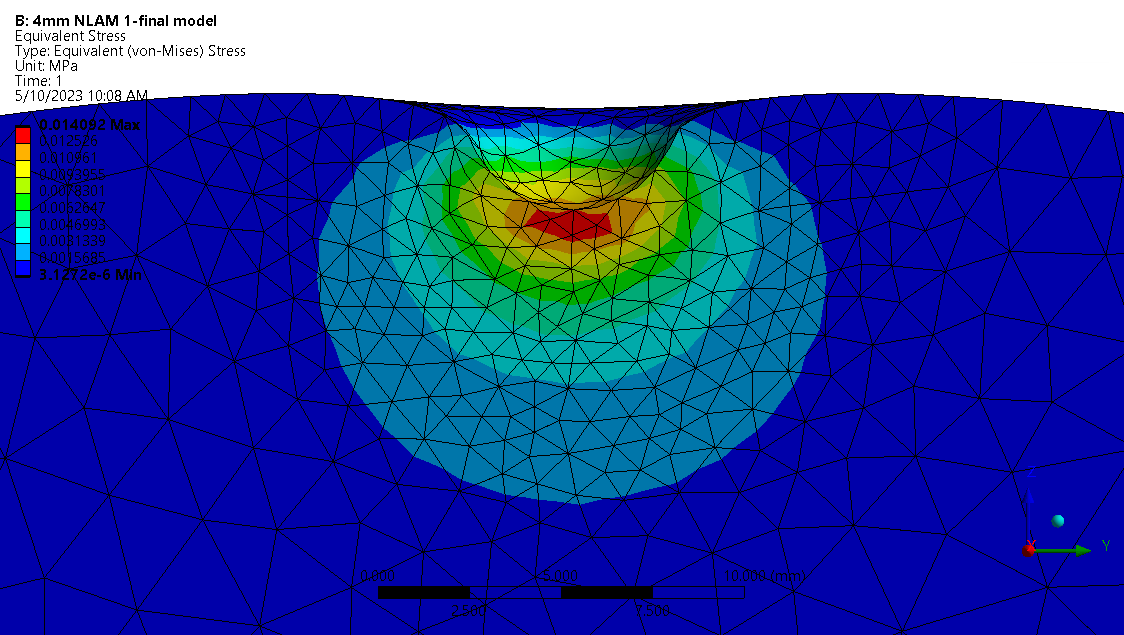
\includegraphics[width=\textwidth]{Images/computational/stresscmII.png}
    \caption{Computational model II}
    \label{fig:cm2stress}
    \end{subfigure}
    \hspace{0.3cm}
    \caption[Stress distribution analysis]{Comparison of stress distribution in computational models I and II with a Neo-Hookean material model after mesh strategy improvements.}
    \label{fig:cmIIstressdistanalysis}
\end{figure}

\subsubsection*{Adjustments to Deformation Behavior}
During the simulated indentation process, an unusual deformation pattern was observed in the computational model.
The indented mass in the model tended to move upwards, enveloping the spherical indenter, which deviated from the 
experimental test observations. In the real-world experiments, the indented mass seemed to 
displace sideways. This discrepancy was attributed to the fixed support boundary condition on the lower specimen's 
surface, which restricted lateral movement of the indented mass.

To improve this unnatural deformation pattern, a more accurate representation of the 
experimental setup was introduced into the FE model. The specimen was positioned on a bowl-shaped
platform, mirroring the experimental configuration. The platform was designed with a slightly major radius to allow 
for lateral displacement of the indented mass to avoid over-constraining the specimen. The contact 
between the specimen and the platform was set to frictional, with a friction coefficient of 0.2, and the base of the platform 
possessed a fixed support.

The inclusion of the platform in the FE model had an impact on the deformation in the indentation area, 
as it showed a more natural deformation. Also, there was an impact on the load-displacement curve (Fig. \ref{fig:noplatformvsplatform}). 
The curve with platform showed a better fit to the experimental data, as the overall shape of the curve was more 
comparable to the experimental data. Therefore, the FE model with the platform was selected as the final model for computational 
model II.\\
\begin{figure}%
    \centering
   \quad
    \begin{tikzpicture}[scale=1]
        \begin{axis}[
            xmax=4,xmin=0,
            ymin= 0,ymax=0.6,
            ytick={0,0.1,0.2,...,0.5},
            xlabel={Displacement $u [mm]$},
            ylabel={Force reaction $F_I [N]$},
            grid = major,
            legend pos= north west]
            \addplot+[smooth, no markers, thick] table [y=$Force$, x=Def]{Table/Middle Point/MPII4mmtotalap.dat};
            \addplot+[smooth, no markers, thick] table [y=$Force$, x=Def]{Table/CP2/CP2noplatNH8541_5.dat};  
            \addplot+[smooth, no markers, thick] table [y=$Force$, x=Def]{Table/CP2/CP2platNH8541_5.dat};            
            \legend{Middle Point, CM II-No platform, CM II-Platform}
        \end{axis}
    \end{tikzpicture}%
   \caption[CP II: No platform vs. with platform]{NBP - CM I vs. EM I: Comparison of force-displacement curves between experimental data for Nearby Point case and the initial computational model with a Neo-Hookean model for $h = \SI{3.8}{\milli \meter}$.}%
   \label{fig:noplatformvsplatform}%
\end{figure}

This chapter has presented an in-depth analysis of the development and refinement of the computational models I and II, used
for simulating the indentation tests. The transition from CM I to CM II revealed the challenges encountered in an indentation 
simulation model and how significant is handling large element deformation for the mesh quality improvement. 
Specifically, the use of a nonlinear adaptive region facilitated more reliable simulation results, displaying a more 
closely Hertzian solution. This improvement reinforced the model's robustness for the subsequent application in an inverse
finite element method approach for the identification of the material's parameters. Moreover, the adjustment in involving platform
emphasized the importance of incorporating realistic boundary conditions and constraints into the computational model.
%best result with convergence
%Their a two main factors which increases the complexity of the validation of the simulation
%and those are, the contact nonlinearity, and the element distortion due to indentation
% experiment. These issues make the computational time expensive, as it requires to manual 
% solutions for the meshing in the area of importance, and small time steps. 
% For that, the nonlinear adaptive meshing option in ANSYS Workbench was applied, which does a remeshing
% process if the a certain parameter is exceeded.%Revisar explanation of nonlinear adaprive meshing
%Specially, for larger indentation cases, this option shows a more stable model with a good mesh convergence analysis.



